% NOTE - this is only a template without real arguments
\begin{entry}{Phase 4 completion}{Dec 31, 2021}
    \objective 
    
    Complete, test, and refactor phase 4. (Note: completed well before this date, just updating the journal)


    \outline

    \begin{itemize}
        \item Determine scheme and method for GO-GSP communications
        \item Establish GOSensor
        \item Write sensor method
        \item Test sensor
        \item Write decision-making method
        \item Test decision-making process
        \item Establish GOOutputInterface
        \item Write method to gather information for service request/feedback
        \item Write method to generate service request messages
        \item Write method to establish/perform communications tasks
        \item Develop and execute synchronous functional test of system
    \end{itemize}

    \procedures

    \section*{Determine scheme and method for GO-GSP communications}
    I was expecting this part in particular to be the most complex part of the system; however, since we'd already
    limited ourself to requiring the ME and GSP to be run on the same system due to the RWHDERS input, we recognized
    that we could do the exact same thing here by allowing communications to be handled by the MC writing, and the GSP
    parsing, text files. Rather than use the customized .csv files, these communications are easily handled by .xml
    which is easily written and parsed by a multitude of programming language libraries.

    The format for each message is based on the messaging requirements as seen in the GSP Implementation Profile. See
    below.

    \section*{Establish GOSensor}
    The GOSensor class was envisioned to function in two modes: a Manual mode in which grid service requests from the
    GSP would be posted at a specific time by user-configured parameters, and an Automatic Mode in which the requests
    are determined in a more "realistic" manner based on grid states.

    After some thought, we determined that only the Manual Mode would be necessary for the current stage of the project.
    This is due to the fact that we are already using carefully controlled situations for specific testing. Including
    the ability to automatically detect and respond to grid events is a function of the Grid Operator; however, the
    EGoT system is designed to create a DER aggregator, the ME tests the EGoT system, and a sophisticated Grid Operator,
    while possible, is beyond the scope of current work. As such, only Manual Mode is necessary for the time being, with
    most logical determinations being made not by the class but by the Test Engineer during system configration and
    eventual log analysis.

    \subsubsection*{Write and test sensor method}
    The class contains a \verb|self.update_sensor_states()| method, but this is currently unused since Automatic mode
    isn't being implemented at this time. It's a placeholder for when that does happen, and can include on-timestep
    functionality to grab grid states from the measurement processor and make the service request decisions.

    Since this isn't currently being implemented, neither will it be tested at this time.

    \subsubsection*{Write decision-making method}
    There is a \verb|self.make_service_request_decision()| method that is called once per timestep. This is an
    encapsulation method that reads the configuration settings to determine if it's in Automatic or Manual mode and
    calls the according method. In the case of Automatic mode, that method is unwritten and so it's a simple pass
    function.

    For manual mode, a seperate method is called: \verb|self.manually_post_service|. This takes the current simulation
    time as an argument and reads the contents of a prewritten, preloaded "service request" file. This file is in .xml
    format and contains all of the data required to post a service, including the designated time and duration.

    When the simulation reaches the designated time, the proper service is read and "posted". That is, the parameters of
    the requested service are packaged in a dictionary and added to the \verb|self.posted_service_list| attribute for
    use by the GO-GSP communications interface.

    In the future, the Automatic mode will read grid states and determine if a service is required and, if so, what
    parameters are required to address the grid issue. The function will then generate a dictionary with information in
    a format identical to the manually inputted Posted Services.

    \subsubsection*{Write RWHDERS processing method}
    This turned out to be extremely simple, since the input files contain direct power values. It just needs to read the
    power from the files and update the input request dictionary once per time step. If the emulators were to instead
    provide "exporting/importing" flags and label plate data, as was expected, the der-em input request method would
    need to be updated to calculate power based on operating parameters.


    \section*{Test decision-making process}
    Testing was completed satisfactorily after the GOOutputInterface was built and partially tested. The input and output
    files corresponded with one another. See below for more details.

    \section*{Establish GOOutputInterface}
    The main purpose of the GOOutputInterface class is to provide a custom API between the MC and the DERMS under test.
    It needs to be specifically designed and customized for the requirements of the DERMS. It could take any number of
    forms with regards to communications, how they're packaged, etc. But in all cases, they take the Posted Service list,
    translate it into data readable by the DERMS, and send it over each timestep so the DERMS knows what grid services
    the GO is requesting at any given time.

    In theory, the GO-GSP communications should be bidirectional. The GO sends the list of services to the GSP, which the
    GSP acknowledges, but it also provides settlement data for use by the Grid Operator for pricing and validation.
    However, in our tests, validation will be performed by the Test Engineer using human analysis on the logs; therefore,
    there was no need at all to actually code a system to do this automatically. The only communications necessary
    are the posted service list from the GO to the GSP.

    Because of this simplification and prior requirements, we decided that the most efficient way to provide the posted
    services to the GSP would be to put them in an .xml file once per time step, updated based on the requirements of
    the Manual Mode file (or automatically generated services later on.) The services are put in a .xml file that the
    GSP (which, recall, is located on the same system) can read and respond to by its own requirements. The results
    end up in the logs.

    In short, the current architecture of the ME's GO is to read an .xml file containing required service parameters,
    parse them at the proper time and place them in dictionaries in the Sensor class, read the dictionaries with the
    Interface class, and repackage the dictionaries back into nearly identical .xml files for the GSP to use. This
    seemingly roundabout method is necessary both to ensure services are occuring at the proper time, and for
    modularity purposes: if the output protocol is changed, the only part of the method that needs be changed is the
    interface message wrapping. No undue coupling has occured.

    \section*{Testing}
    As with phase 3, full test plan testing requires a functional GSP for full-loop operations. We tested the system
    as fully as possible without the GSP, and found that it seems to function as required.


    \parameters
    
    N/A

    \observations

    RWHDERS turned out to be simple since we made some comprimises with the GSP team to simplify interactivity. Both
    systems can easily generate, read, or parse text files, and the nature of the data is so simple that it makes sense
    to just come up with a scheme for ourselves. This does limit the ME to a new requirement: it must be run on the
    same system as the GSP program; though, we were largely expecting that anyways and there's not a compelling reason
    to run them on seperate systems in the first place.


    \data

    \begin{figure}{gogsp}[H]
        \centering
        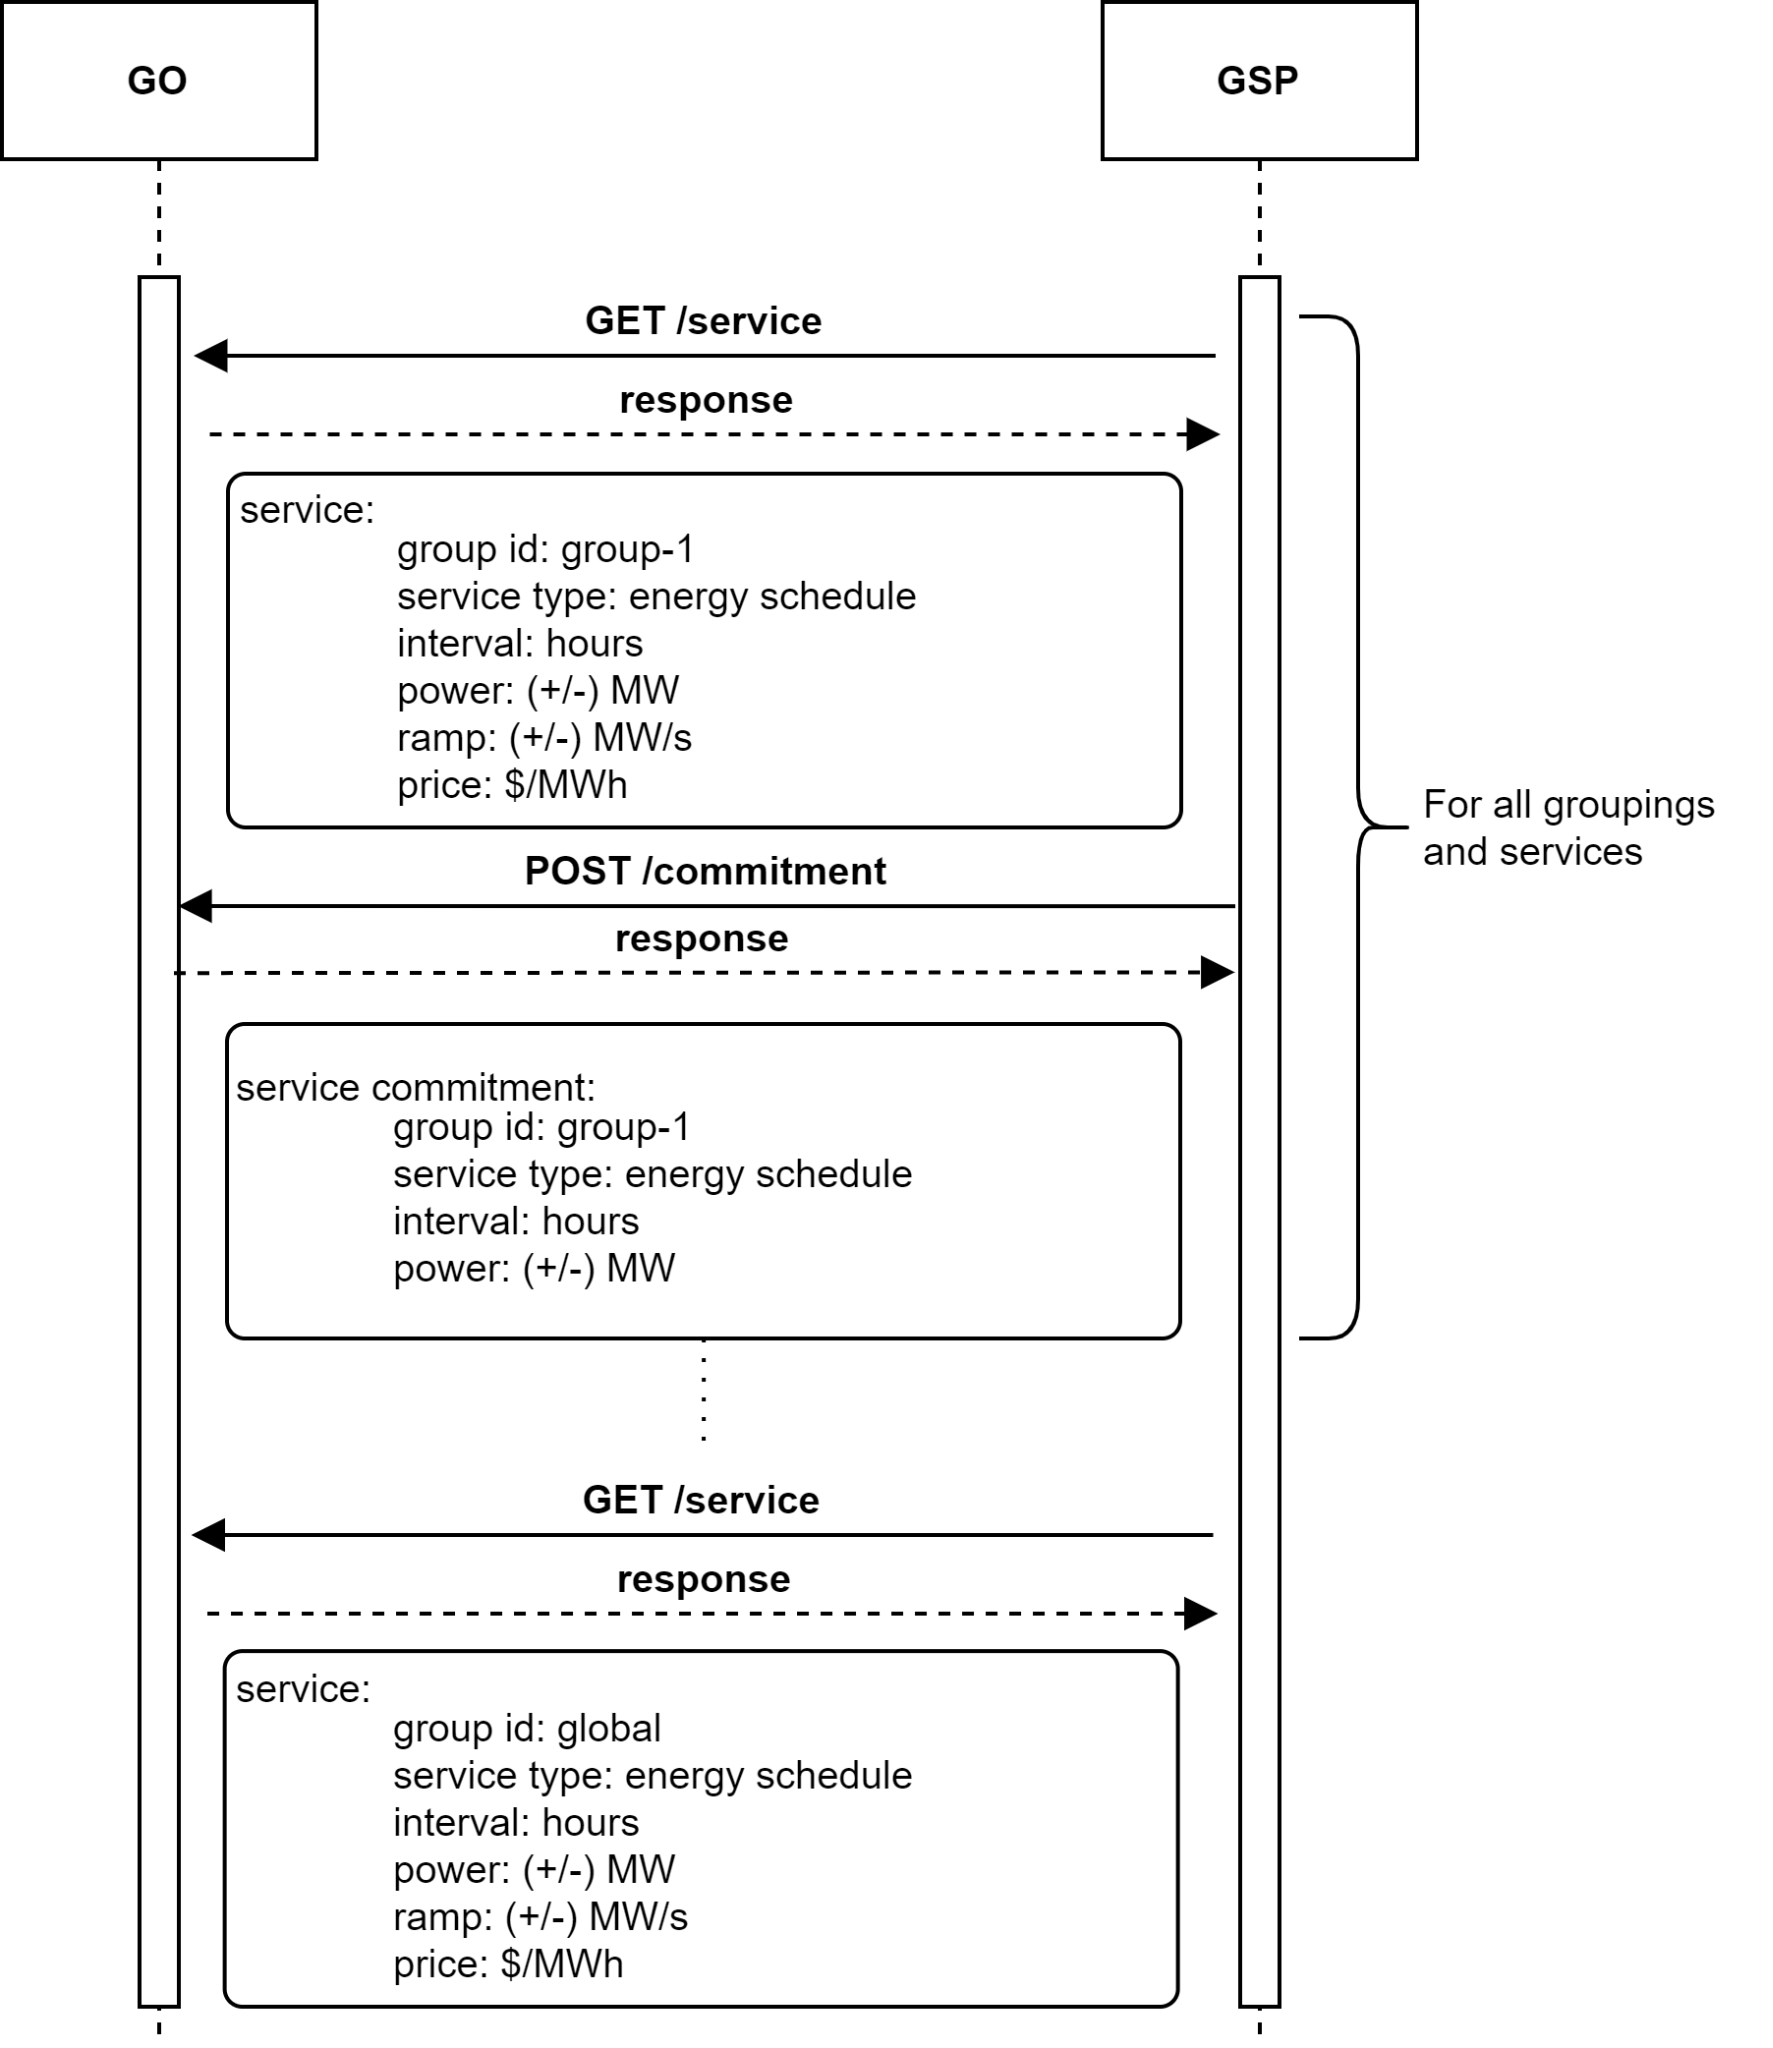
\includegraphics[height=4in]{Fall2021/Figures/goGspcomms}
        \label{fig:gogsp}
    \end{figure}

    Most of the relevent data can be found in the logs. The .xml input and output files are in the ME main folder in
    the GitHub.

    The individual dictionaries communicated from actor to actor are manipulated using complex and often repetitious
    methods. To see the contents of a dictionary at a given simulation time, the best way to go about it is to add
    a print() function to the code and read it in the terminal.

    \results
    
    ME reaches 1.0 pending testing. GSP and ME functional testing will occur in tandem when the GSP is further developed.


\end{entry}


%\begin{entry}{CMake Error running EGOT-DCM Dockerfile}{Dec 02, 2020}
%    \objective
%
%    Determine the cause of the CMake error while running the dockerfile and modify file to get it to successfully build.
%
%    \outline
%
%    \begin{itemize}
%        \item Try running to see if it was just Lorry or a machine issue.
%        \item If it is a machine issue, modify configurations to ensure interoperability.
%        \item If I get the error track down its cause and modify dockerfile to fix.
%        \item Repeat until all builds are successful.
%    \end{itemize}
%
%    \procedures
%
%    \begin{itemize}
%        \item \mint{console}|git clone https://github.com/EGoT-DCS-SunSpec-Modbus|
%        \item \mint{console}|docker build -f Dockerfile.buster -t egot-dcs .|
%        \item \mint{console}|docker container run -i egot-dcs|
%    \end{itemize}
%
%    \observations
%
%    \begin{error}{Cmake Error: No CMAKE\_CXX\_COMPILER found}
%        \begin{figure}[H]
%            \centering
%            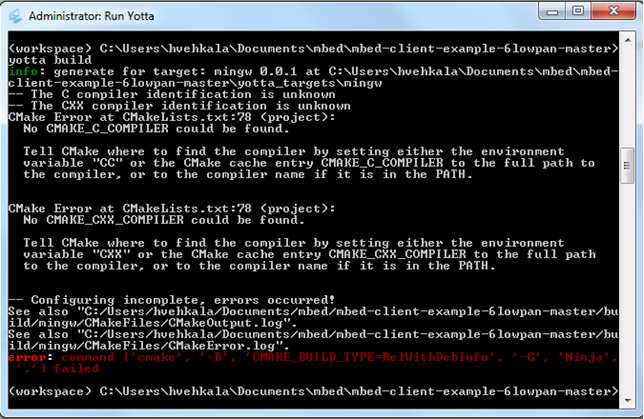
\includegraphics[height=4in]{Fall2020/Figures/cmake_error.png}
%        \end{figure}
%
%        Solution: what you need to do found at \cite{CMAKE-Forum}
%    \end{error}
%
%    \results
%
%    Short: No.
%
%    Long: Well...
%
%
%\end{entry}